
\subsection{Introduction to convex optimization problems}
General form: Consider the functions $F_i(x), h_i(x): \reals^n\rightarrow \reals$.
\begin{align*}
\min_{x\in \reals^n} \quad &F_0(x) \quad \text{"objective function"}\\
s.t. \quad &F_i(x) \leq 0, i = 1...m \quad\text{inequality constraints}\\
&h_i(x) =0,i =1...p \quad \text{equality constraints}
\end{align*}


Feasible set for this question:
$$\mathcal{C} = \{x\vert F_i(x) \leq 0,i=1...m,h_i(x) = 0,i = 1...p \}$$


Optimal value: $p^* = \inf_{x\in \mathcal{C}}F_0(x)$. Note that it could be $\infty$, and also could be empty.

Optimal points: $\{x\in \mathcal{C}\vert F_0(x) = p^* \}$. Note that it could be empty, and also could be not unique.



\begin{example}
Consider the optimization problem:
\begin{align*}
\min_x \quad &\min x_1 + x_2 \\
s.t. 
&-x_1\leq 0\\
&-x_2\leq 0\\
&1- x_1 x_2\leq 0\\
\end{align*}

So $x^*=
\begin{bmatrix}
1\\
1
\end{bmatrix}$
and $p^* = 2$, as illustrated in the figure.

\end{example}


\vspace{0.5cm}
\textbf{Convex optimization problem: }
\begin{align*}
\min_x \quad &F_0(x) \\
s.t. &F_i(x)\leq 0 \quad i = 1,\cdots,m\\
&a^T_i x - b_i = 0 \quad i =i,\cdots,p\\
\end{align*}
$a^T_i + b_i = 0$ is often written as:
$$
\begin{bmatrix}
a_1^T\\
a_2^T\\
\vdots\\
a_p^T
\end{bmatrix}x = 
\begin{bmatrix}
b_1\\
\vdots\\
b_P
\end{bmatrix}
\Leftrightarrow
Ax=b
$$

\begin{enumerate}
	\item All $F_i$, $i\in \{0,1,...n \}$ are convex functions.
	\item All equality constraints are affine.
\end{enumerate}


%\begin{example}
%	\begin{align*}
%	&\min\quad{x_1+x_2}\\
%	s.t. &-x_1\leq 0\\
%	&-x_2\leq 0\\
%	&1-x_1x_2 \leq 0\\
%	\end{align*}
%	
%	GRAPH7
%\end{example}

\textbf{Remarks:}
\begin{enumerate}
	\item Think about feasible set,
	\begin{equation*}
	\mathcal{C} = ( \cap^m_{i=1}\{x\vert F_i(x) \leq 0 \} ) \cap (\cap^p_{i=1}\{x\vert a_i^Tx - b_i = 0 \})
	\end{equation*}
	
	For the first part, each is a sublevel set of a convex function therefore convex.
	
	For the second part, each is an affine set and therefore convex.
	
    So the feasible set $\mathcal{C}$ is an intersection of $p+m$ convex sets, and therefore it is a convex set.
	
	\item Note: $h_i(x)$ are affine(and not more general convex) to keep the set $\{x\vert h_i(x) = 0 \}$ a convex set. 
	
	Let $h_i(x) = x^2 - 1$: 
	\begin{equation*}
	\{x\vert x^2 - 1 = 0 \} = \{x\vert x^2 = 1 \} = \{\pm 1 \}
	\end{equation*}
	\begin{marginfigure}
	\centering
	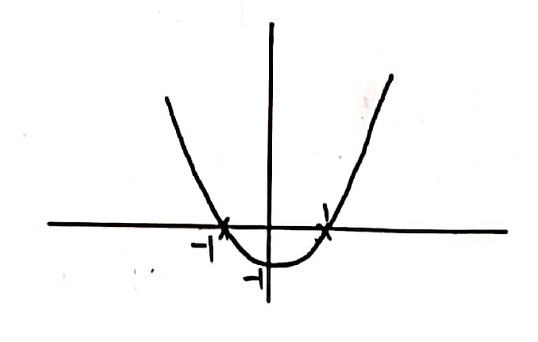
\includegraphics[width=1.8in,height=1.8in]{figures/ch08/figure1111_6.png}
	%\caption{This is an inserted JPG graphic} 
	%\label{fig:graph} 
	\end{marginfigure}
\end{enumerate}

%Above are notes for Nov 11


%Below are notes for Nov 13

\begin{align*}
\min_x\quad & F_0(x) \\
s.t.\quad & F_i(x) \leq 0 \quad i = 1,...,m\\
& a_i^Tx - b_i = 0\quad i = 1,...,p
\end{align*}

\begin{itemize}
	\item $F_o, F_1,...,F_m$ are convex
	
	\item $Ax - b = 0$
\end{itemize}

\begin{definition}
	$x\in \mathcal{C}$ is locally optimal for a constrained optimization if $\exists \epsilon > 0$, $s.t.\forall y\in \mathcal{C}$ and $\Vert x-y\Vert < \epsilon$, we have $F_0(y) \geq F_0(x)$
\end{definition}

\begin{theorem}
	For a convex optimization problem a local minimum is global optimization. 
\end{theorem}
Proved aparticular instance of this for:
\begin{enumerate}
	\item Unconstrained optimization
	
	\item Differentiable $F_0$
\end{enumerate}

\begin{proof}
	(Proof by contradiction)
	
	Suppose $x\in \mathcal{C}$ is not globally optimal but is locally minimal.
	
	$\rightarrow$ Because not globally optimal, $\exists y\in \mathcal{C}$ s.t. $F_0(y)<F_0(x)$
	
	$\rightarrow$ Consider $z = \lambda x + (1-\lambda)y\in \mathcal{C}$ because $\mathcal{C}$ is convex.
	
	\begin{align*}
	F_0(z) &\leq \lambda F_0(x) + (1-\lambda)F_0(x)\\
	&< \lambda F_0(x) + (1-\lambda)F_0(x)\\
	&= F_0(x)
	\end{align*}
	
	$\rightarrow$ By picking $\lambda$ sufficiently close to 1(but $<$ 1), $z\in \mathcal{C}$ is in neighborhood of $x$ and has lower cost so $x$ cannot be local minimum. $\Rightarrow$ Contradiction
\end{proof}

As for: 

\begin{align*}
\min_x\quad & F_0(x) \\
s.t.\quad & F_i(x) \leq 0 \quad i = 1,...,m\\
& a_i^Tx - b_i = 0\quad i = 1,...,p
\end{align*}


For differentiable convex $F_0$:

\begin{itemize}
	\item For unconstrained $x^*$ is optimal iff $\triangledown F(x^*) = 0$
	
	\item For constrained optimization very possible no $x\in \mathcal{C}$ satisfies $\triangledown F(x) = 0$
\end{itemize}

\begin{theorem}
	For a convex optimization problem with (convex) feasible set $\mathcal{C}$ and differentiable (convex) objective $F_0: \Re^n \rightarrow \Re_i$, a point $x^* \in \mathcal{C}$ is optimal iff:
	
	\begin{equation*}
	\triangledown F_0(x)^T(y - x^*) \geq 0  \quad \forall y \in \mathcal{C}
	\end{equation*}
\end{theorem}

Start at positive optimum $x^*\in \mathcal{C}$, move into feasible set in direction $v$ and evaluate, $F_0(x^*+tv)$ must be non-decreasing for $t\geq 0$.

\begin{marginfigure}
\centering
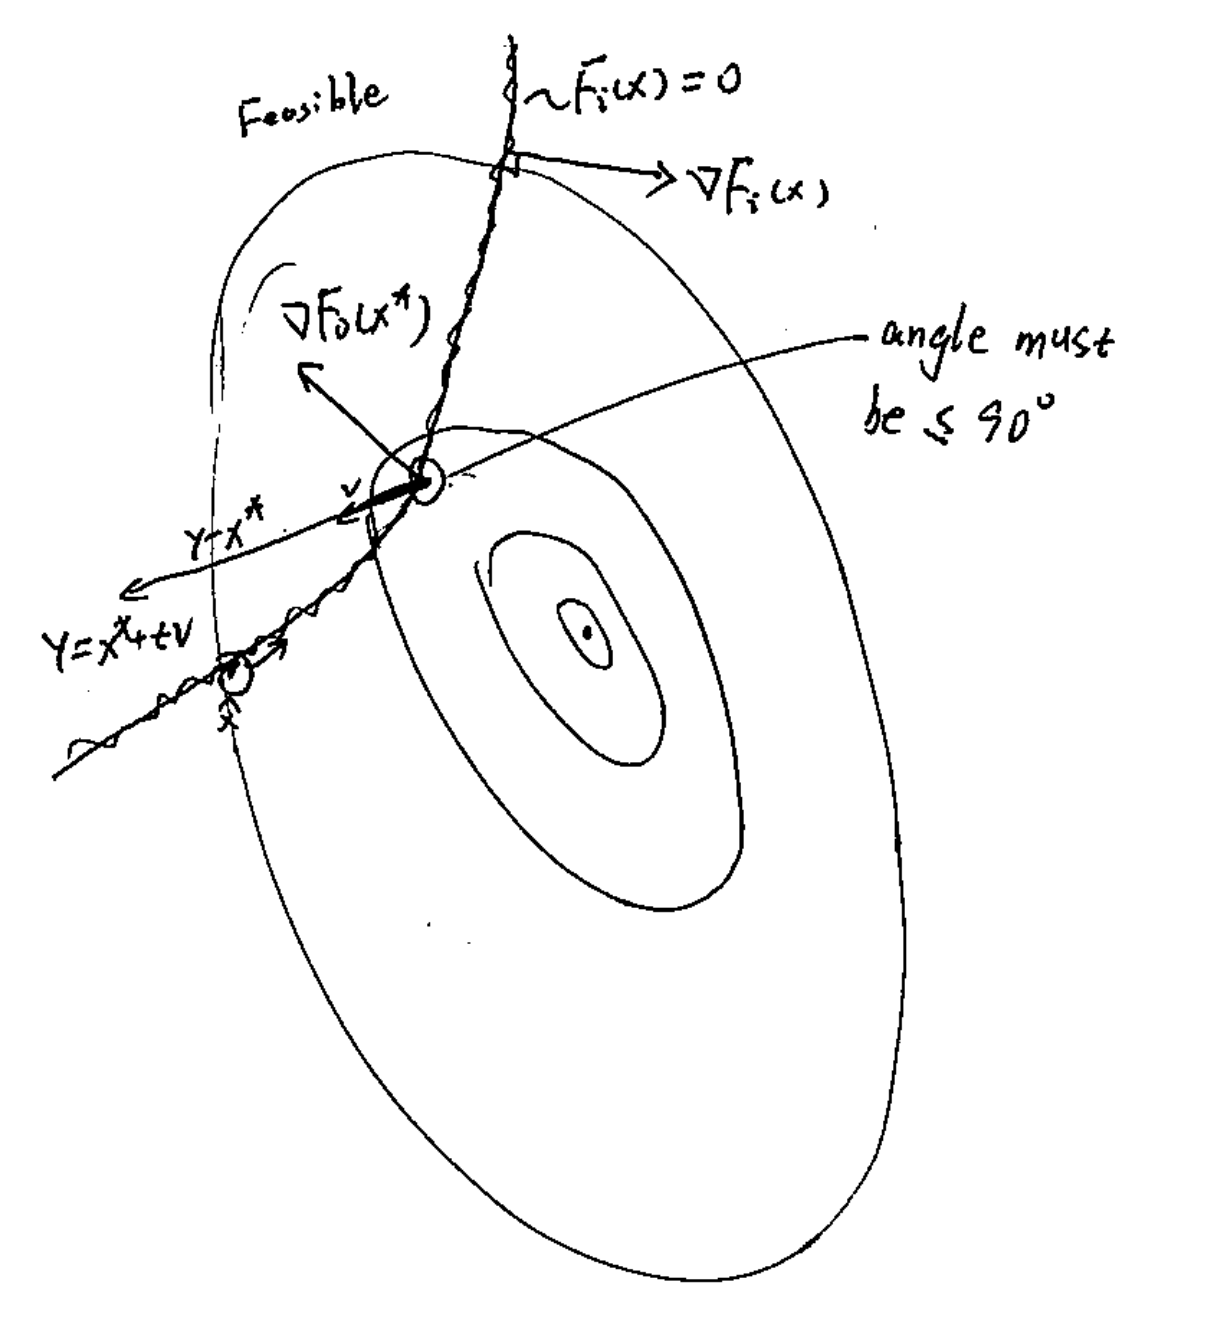
\includegraphics[width=1.8in,height=1.8in]{figures/ch09/figure1113_1.png}
%\caption{This is an inserted JPG graphic} 
%\label{fig:graph} 
\end{marginfigure}

\begin{proof}
	First assume $x^*$ is the global optimum, apply $1^{st}$-order condition for optimality, i.e. $\forall y \in \mathcal{C}$:
	
	\begin{align*}
	F_0(y) &\geq F_0(x^*) + \triangledown F_0(x^*)^T(y-x^*)\\
	&\geq F_0(x^*)
	\end{align*}
	$\rightarrow$ Basically same prove now $2^{nd}$ term $\geq 0$(not = 0)
	
	Second: 
	
	If $x^*$ is global optimum, suppose $x^*$ is global optimum and $\exists y\in \mathcal{C}$s.t. $\triangledown F_0(x^*)^T(y-x^*)<0$.
	
	Look at points 
	
	\begin{align*}
	z &= \lambda y + (1-\lambda)x^*\\
	&= x^* + \lambda(y-x^*)\quad \lambda \in [0,1]
	\end{align*}
	Feasible $\forall \lambda$ because $\mathcal{C}$ is convex set.
	
	\begin{align*}
	\left.\frac{dF_0(z)}{d\lambda}\right|_{\lambda = 0} &=\left.\frac{d}{d\lambda}F_0(x^*+\lambda(y-x^*))\right|_{\lambda = 0}\\
	&= \triangledown F_0(x^*)^T(y-x^*)\\
	&< 0
	\end{align*}
	
	Since slope is strictly negative, as increasing $\lambda>0$, initially $F_0(z)$ decreases $\rightarrow$ contradicts global optimality of $x^*$, therefore have a contradiction. 
\end{proof}


\subsection{Quasi-convex minimization}

Recall: $F_0$ is quasi-convex if all its sub-level sets are convex sets

Problem:


\begin{align*}
\min_x\quad & F_0(x) \quad \leftarrow \text{quasi-convex}\\
s.t.\quad & F_i(x) \leq 0 \quad i = 1,...,m \quad \leftarrow \text{convex}\\
& a_i^T - b_i = 0\quad i = 1,...,m \quad \leftarrow \text{affine}
\end{align*}

can be written as:


\begin{align*}
\min_x\quad & F_0(x) \quad \leftarrow \text{convex set}\\
s.t.\quad  & F_0(x) \leq t  \\
& F_i(x) \leq 0 \quad i = 1,...,m \\
& a_i^T - b_i = 0\quad i = 1,...,m
\end{align*}
which is a feasible problem

\begin{example}
	$F_0(x) = \frac{P(x)}{Q(x)}$ where $p(x)$ is convex, $q(x)$ is concave, $domF_0 = \{x\vert Q(x) >0 \}$.
	
	\begin{align*}
	\{x\vert F_0(x) \leq t \} &= \{x\vert \frac{P(x)}{Q(x)}\leq t \}\\
	&= \{x\vert P(x)\leq tQ(x) \}\\
	&= \{x\vert P(x) - tQ(x)\leq 0 \}\\
	f_0(x) &= \frac{a^Tx + b}{c^Tx+d}
	\end{align*}
	
	If the $P(x) - tQ(x)$ is convex, then $f_0$ us quasi-convex.
	
	\begin{itemize}
		\item super-level set convex $\Rightarrow$ quasi-concave
		
		\item sub-level set convex $\Rightarrow$ quasi-convex
	\end{itemize}
	
	Quasi-convex promises a global optimal
\end{example}

Generalized inequalities:

\begin{align*}
\min_x\quad & F_0(x) \\
s.t.\quad & F_i(x) \leq_{k_i} 0 \quad i = 1,...,m\\
& h_i(x) = 0\quad i = 1,...,m 
\end{align*}
where $F_0(x): \Re^n\rightarrow \Re$ convex, $F_i: \Re^n\rightarrow \Re^l$ "$K_i$-convex", $k_i$ are cones.

\begin{equation*}
	F_i(\lambda x + (1-\lambda)y)\leq_{k_i} \lambda F_i(x) + (1-\lambda)F_i(y)
\end{equation*}\\

Semi-definite program:
\begin{align*}
\min_x\quad & c^Tx \\
s.t.\quad & A_0+A_1x_1+,,,+A_nx_n\leq 0\quad \text{"LMI": linear matrix inequlity}\\
& Fx = g
\end{align*}
where $-(A_0+A_1x_1+,,,+A_nx_n)\in S^n$, $A_i\in S^n$, $\leq$ means they're PSD matrices.
%Above are notes for Nov 13


%Below are notes for Nov 18


%Above are notes for Nov 18
